\section{Metodologia}\label{sec-metodologia}

\subsection{Instrumentos de pesquisa}

Para a responder às perguntas de pesquisa e alcançar o objetivo deste
estudo, foram realizados três experimentos com 81 alunos com nível
elementar de proficiência em língua inglesa cursando o 1º ano do ensino
médio. Os experimentos foram feitos em 2024 no colégio de aplicação de
uma universidade pública de Minas Gerais. Todos os participantes foram
submetidos aos mesmos instrumentos de pesquisa (\Cref{tab-01}), com exceção
do ambiente de aprendizagem, o qual variou de acordo com a condição de
testagem. Esta pesquisa foi aprovada pelo Comitê de Ética em Pesquisa
CEP/UFJF sob o CAAE 71129823.6.0000.5147.

\begin{table}[htpb]
    \centering
    \begin{threeparttable}
    \caption{Instrumentos de pesquisa e seus respectivos objetivos.}
    \label{tab-01}
        \begin{tabular}{p{.475\textwidth} p{.475\textwidth}}
            \toprule
            Instrumento de pesquisa & Objetivo \\
            \midrule
            Teste de proficiência & Avaliar a proficiência linguística dos
            participantes. \\
            Pré-teste de vocabulário & Identificar a familiaridade dos participantes
            com as palavras alvo do experimento. \\
            Questionário de identificação & Traçar o perfil dos participantes. \\
            Ambientes de aprendizagem & Expor os alunos às palavras alvo do
            experimento por meio diferentes modalidades. \\
            Pós-teste de vocabulário & Mensurar quantitativamente a aprendizagem das
            palavras alvo após a exposição aos ambientes. \\
            Questionário de avaliação da experiência & Mensurar a opinião dos
            participantes sobre a experiência de aprendizagem de vocabulário nos
            ambientes e sua contribuição (ou não) para promover a motivação e a
            atenção. \\
            \bottomrule
        \end{tabular}
    \source{Elaborado pelas autoras (2024).}
    \end{threeparttable}
\end{table}

O estudo se organizou em três etapas: pré-testagem, testagem e
pós-testagem. Na primeira etapa, foi aplicado a todos os participantes o
pré-teste de vocabulário, o teste de nivelamento e o questionário de
identificação. Na segunda etapa, cada grupo com 27 alunos foi exposto a
um dos ambientes: ambiente imersivo em 360º, ambiente de leitura com
glossário multimodal e ambiente imersivo em 360º + ambiente de leitura
com glossário multimodal. Na terceira etapa, foi aplicado aos
participantes o pós-teste imediato de vocabulário e um questionário de
avaliação da experiência. A seguir, os três ambientes usados serão
melhor detalhados.


\subsection{Ambientes utilizados para geração de dados }\label{subs-sec-ambientesutilizados}

Ferramentas digitais estão cada vez mais presentes em nosso dia a dia,
devendo ser incorporadas também ao ambiente educacional. Contudo, em
contextos de baixo investimento em educação, como é o caso do Brasil,
isso é dificultado, pois o uso de tecnologias, como a realidade virtual
(RV), implica um alto custo, visto que requerem uma especialização muito
além do conjunto de habilidades dos professores e da precária
infraestrutura das escolas públicas. Uma alternativa é o uso de
dispositivos tecnológicos que são próximos à RV, porém mais acessíveis,
como as imagens 360º. Neste sentido, à luz das teorias que embasam este
estudo, selecionamos e adaptamos um ambiente imersivo de aprendizagem,
bem como criamos um ambiente de leitura para responder às perguntas que
guiam esta pesquisa e investigar o papel da multimodalidade como
potencial recurso para promover atenção e motivação durante a
aprendizagem de vocabulário de LE.

Adaptamos um ambiente de RV da plataforma \emph{Avanti\textquotesingle s
World}\footnote{O ambiente imersivo da plataforma \emph{Avanti's World}
  encontra-se disponível em
  \url{https://www.avantisworld.com/}{https://www.avantisworld.com}.}
para usá-lo o como um ambiente imersivo em 360º, facilitando sua
aplicação através dos \emph{desktops} da escola em que os experimentos
foram realizados. Selecionamos uma amostra cujo cenário é a casa da
família Capuleto, da peça Romeu e Julieta, por conta da popularidade da
peça e provável familiaridade dos alunos com ela. Esse cenário se divide
em três cenas: \emph{The orchard}, \emph{Juliet's bedroom} e \emph{The
Capulet's tomb} (\Cref{fig-01}). Em cada cena, há objetos em 360º que possuem
um papel central na trama, como o veneno e a adaga presentes na última
cena, diretamente relacionados ao desfecho trágico da trama.

\begin{figure}[htpb]
    \centering
    \begin{minipage}{.75\textwidth}
    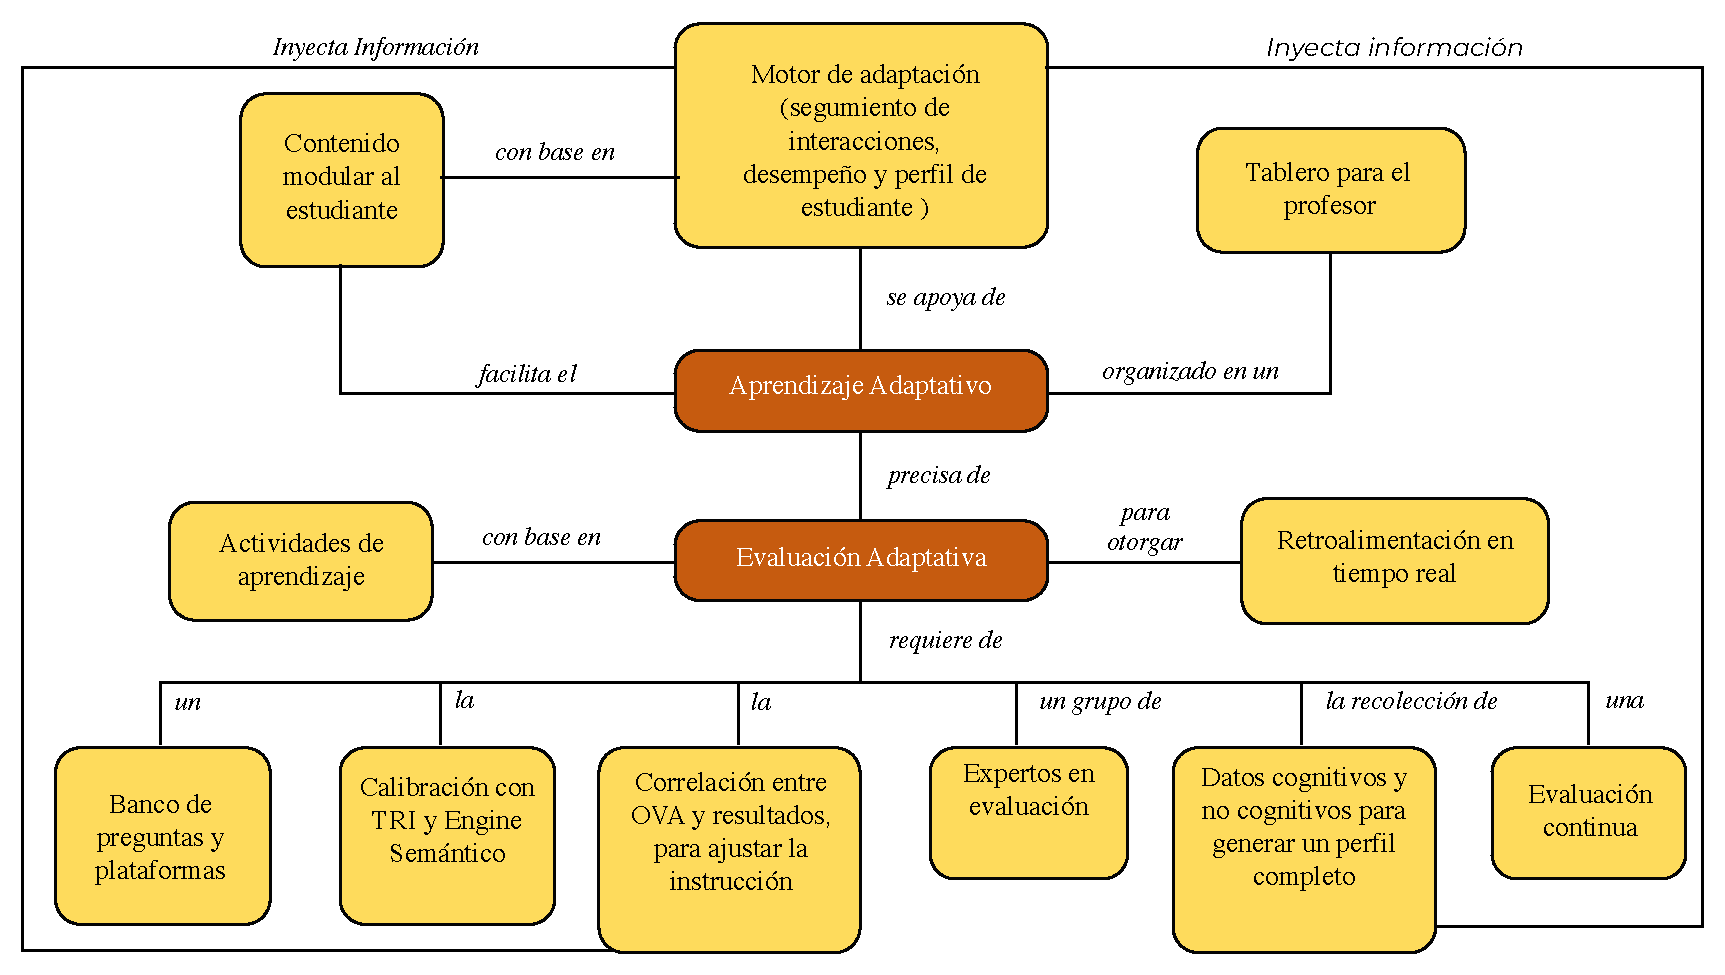
\includegraphics[width=\textwidth]{fig-01.png}
    \caption{Cena \emph{The Capulet's tomb} vista de um ângulo.}
    \label{fig-01}
    \source{\url{https://www.avantisworld.com/}
    (2024).}
    \end{minipage}
\end{figure}

Apesar de ser a melhor alternativa encontrada para tornar o uso da RV
mais acessível às escolas, esse ambiente possui limitações, por exemplo,
não permitir a inserção de um glossário multimodal em sua interface, o
que possibilitaria a consulta do significado e da pronúncia das palavras
alvo simultaneamente à exploração do ambiente, além de oferecer apoio
verbal aos alunos.

Para suprir tal limitação, foi elaborado um ambiente de leitura com
glossário multimodal com base nos estudos de \textcite{souza2004}, \textcite{saito2015}
e \textcite{procopio2016} sobre aprendizagem implícita de vocabulário em
ambiente multimodal. Segundo \textcite{procopio2016}, o uso do glossário
multimodal proporciona exposição a insumo linguístico compreensível,
contribuindo para realização de inferências mais precisas e retenção do
vocabulário inferido. Para a elaboração desse ambiente, manteve-se a
mesma temática literária do ambiente imersivo 360º e foi utilizada a
plataforma \emph{Wix Website} para criar um site\footnote{Disponível em:
  \url{https://rafaelalemos834.wixsite.com/my-site}}. Nele, foram
inseridas informações sobre os personagens principais da peça Romeo e
Julieta e um resumo dessa história em forma de hipertexto (\Cref{fig-02}),
cujos \emph{links} são palavras alvo do experimento e direcionam os
alunos ao glossário multimodal (\Cref{fig-03}), o qual oferece a definição, a
representação imagética e a pronúncia dessas palavras.

\begin{figure}[htpb]
    \centering
    \begin{minipage}{.75\textwidth}
    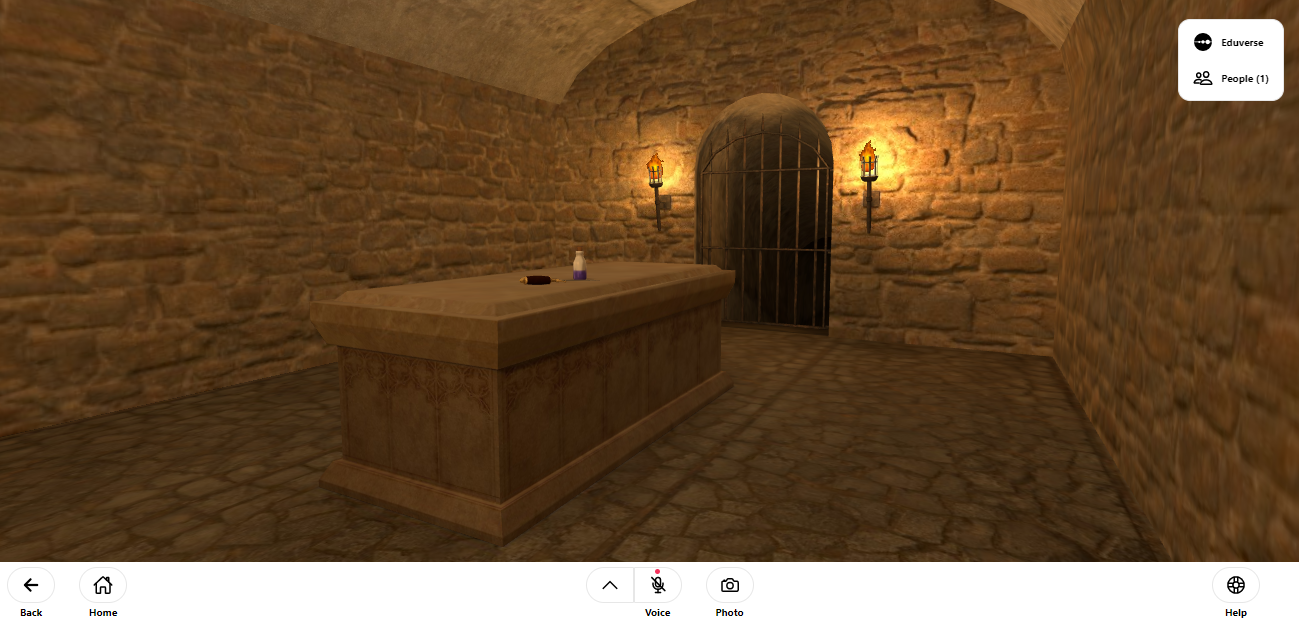
\includegraphics[width=\textwidth]{fig-02.png}
    \caption{Hipertexto Romeu e Julieta.}
    \label{fig-02}
    \source{\url{https://rafaelalemos834.wixsite.com/my-site}
    (2024).}
    \end{minipage}
\end{figure}

\begin{figure}[htpb]
    \centering
    \begin{minipage}{.75\textwidth}
    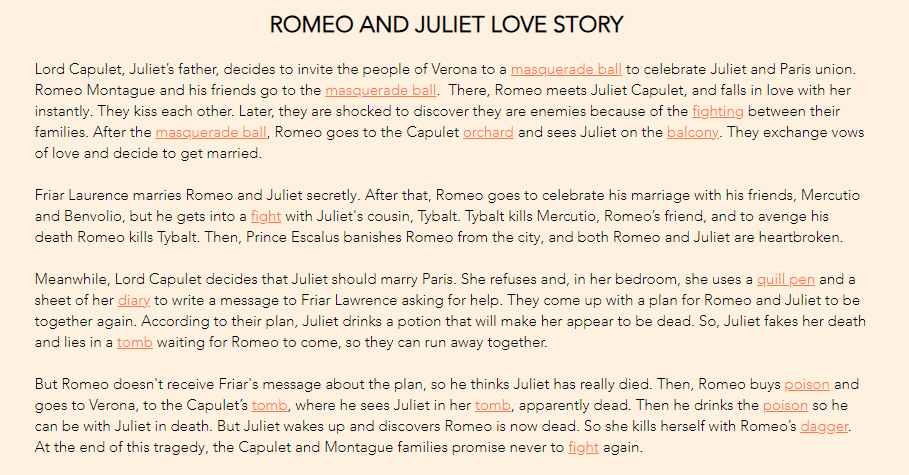
\includegraphics[width=\textwidth]{fig-03.png}
    \caption{Glossário multimodal presente no ambiente de leitura.}
    \label{fig-03}
    \source{\url{https://rafaelalemos834.wixsite.com/my-site}
    (2024).}
    \end{minipage}
\end{figure}
Ainda, criou-se um terceiro ambiente, no qual os dois anteriormente
mencionados (ambiente imersivo em 360º e ambiente de leitura com
glossário multimodal) foram integrados. Essa combinação permite suprir
algumas lacunas presentes em cada um dos dois ambientes, como a falta de
suporte escrito no ambiente imersivo.

Com os instrumentos de pesquisa explicitados, sobretudo os ambientes
utilizados neste estudo, a seguir, serão discutidos os experimentos
realizados e os dados obtidos.
